% !TEX root =  ../main_manuscript.tex

\subsection{Study Population}
\label{subsec:study_population}
To develop our methodology we use the data of prostate cancer patients from the world's largest AS study called PRIAS \cite{bokhorst2016decade} (see Table \ref{table:prias_summary}). More than 100 medical centers from 17 countries worldwide contribute to the collection of data, utilizing a common study protocol and a web-based tool, both available at \url{www.prias-project.org}. We use data collected over a period of ten years, between December 2006 (beginning of PRIAS study) and December 2016. The primary event of interest is cancer progression detected upon a positive biopsy. The time of cancer progression is interval censored because biopsies are scheduled periodically. Biopsies are scheduled as per the PRIAS protocol (see \hyperref[sec:introduction]{Introduction}). There are three types of competing events, namely death, removal of patients from AS on the basis of their observed DRE and PSA measurements, and loss to follow-up. We assume these three types of events to be censored observations (see Appendix~A.5 for details). However, our model allows removal of patients to depend on observed longitudinal data and baseline covariates of the patient. Under the aforementioned assumption of censoring, Figure~\ref{fig:npmle_plot} shows the cumulative risk of cancer progression over the study follow-up period.

\begin{table}
\captionsetup{justification=justified}
\small\sf\centering
\caption{\textbf{Summary statistics for the PRIAS dataset}. The primary event of interest is cancer progression. A DRE measurement equal to T1c\cite{schroder1992tnm} indicates a clinically inapparent tumor which is not palpable or visible by imaging, while tumors with $\mbox{DRE} > \mbox{T1c}$ are palpable. The abbreviation IQR means interquartile range.}
\label{table:prias_summary}
\begin{tabular}{lr}
\toprule
Data & Value\\
\midrule
Total patients & 5270\\
Cancer progression (primary event) & 866\\
Loss to follow-up (anxiety or unknown) & 685\\
Patient removal on the basis of PSA and DRE & 464\\
Death (unrelated to prostate cancer) & 61\\
Death (related to prostate cancer) & 2\\
\midrule
Median Age (years) & 70 (IQR: 65--75)\\
Total PSA measurements & 46015\\
Median number of PSA measurements per patient &  7 (IQR: 7--12)\\
Median PSA value (ng/mL) & 5.6 (IQR: 4.0--7.5)\\
Total DRE measurements & 25606\\
Median number of DRE measurements per patient & 4 (IQR: 3--7)\\
$\mbox{DRE} = \mbox{T1c}$ (\%) & 23538/25606 (92\%) \\
\bottomrule
\end{tabular}
\end{table}

\begin{figure}[!htb]
\captionsetup{justification=justified}
\centerline{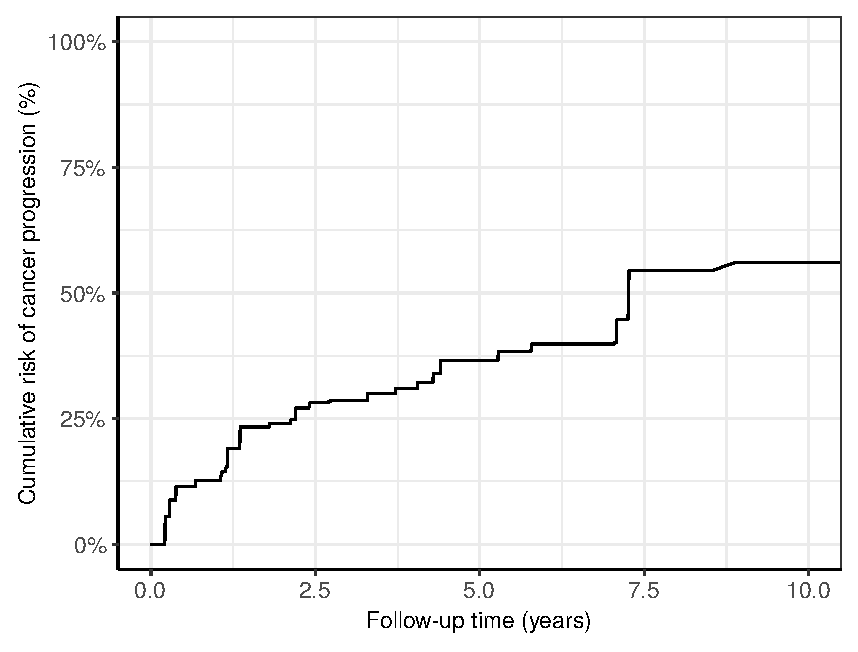
\includegraphics[width=\columnwidth]{images/npmle_plot.eps}}
\caption{\textbf{Estimated cumulative risk of cancer progression in AS} for patients in the Prostate Cancer Research International Active Surveillance (PRIAS) dataset. Nearly 50\% patients (\textit{slow progressing}) do not progress in the ten year follow-up period. Cumulative risk is estimated using nonparametric maximum likelihood estimation \citep{turnbull1976empirical}, to account for interval censored cancer progression times observed in the PRIAS dataset. Censoring includes death, removal from AS on the basis of observed longitudinal data, and patient dropout.}
\label{fig:npmle_plot}
\end{figure}

For all patients, PSA measurements (ng/mL) are scheduled every 3 months for the first 2 years and every 6 months thereafter. The DRE measurements are scheduled every 6 months. We use the DRE measurements as $\mbox{DRE} = \mbox{T1c}$ versus $\mbox{DRE} > \mbox{T1c}$. A DRE measurement equal to T1c\cite{schroder1992tnm} indicates a clinically inapparent tumor which is not palpable or visible by imaging, while tumors with $\mbox{DRE} > \mbox{T1c}$ are palpable.

\textbf{Data Accessibility:} The PRIAS database is not openly accessible. However, access to the database can be requested on the basis of a study proposal approved by the PRIAS steering committee. The website of the PRIAS program is \url{www.prias-project.org}.


